\chapter{Sistema binario e rappresentazione dei numeri}
\label{sec:sistema_binario}

Anche se in linea di principio questo non è l'unico approccio possibile,
praticamente tutti i calcolatori moderni funzionano in logica binaria---cioè
manipolano e conservano i dati al loro interno sotto forma di \foreign{bit}, o celle
elementari di memoria che possono assumere uno due valori possibili
(convenzionalmente $0$ o $1$). Questo deriva essenzialmente dal fatto che i
dispositivi di memorizzazione più diffusi si basano, a livello elementare, sul
\foreign{flip-flop}, che è un circuito elettronico a due stati.

In questa appendice ci occupiamo brevemente della rappresentazione dei numeri
in un calcolatore e dei problemi numerici che si incontrano tipicamente
nell'aritmetica in virgola mobile.


\section{Una piccola provocazione}

Guardiamo per un attimo il frammento di codice~\ref{snip:floating_point}:
sorprendente, vero? L'aritmetica in virgola mobile è sempre una sorgente copiosa di
sorprese per chi si avvicina per la prima volta alla
programmazione~\cite{python_floating_point, bush_floating_point}, e lo scopo
principale di questa appendice è di affrontare il problema nei termini più
semplici possibili.

\snip[0.55]{floating_point}{%
Semplici esempi di aritmetica in virgola mobile che mettono in luce alcuni
dei problemi tipici che si presentano nel calcolo scientifico.
Vale la pena sottolineare che l'inesattezza dell'aritmetica in virgola mobile
è una proprietà intrinseca dei calcolatori digitali (i.e., non è una
caratteristica di \python, anche se linguaggi diversi hanno possono avere
idiosincrasie diverse).
}

La questione fondamentale è tutto sommato ovvia: la maggior parte dei numeri
reali non ha uno sviluppo decimale (o uno sviluppo in qualsiasi base) finito,
e i calcolatori non hanno memoria (sia essa volatile o persistente) infinita,
per cui in generale non è possibile rappresentare esattamente un numero reale
in un calcolatore digitale. In altre parole:
\emph{l'aritmetica in virgola mobile su un calcolatore digitale è, per sua
natura, inesatta, e non garantisce le proprietà elementari che diamo spesso
per scontate (e.g., la proprietà associativa della somma o la proprietà
distributiva della moltiplicazione rispetto alla somma).}
Ma per capire \emph{esattamente} cosa succede nel frammento~\ref{snip:floating_point}
dobbiamo prima imparare a contare in base $2$\ldots


\section{Sistemi di numerazione in base diversa da 10}

Quando scriviamo il numero $127$ (nella consueta notazione posizionale in base
$10$) quello che in effetti intendiamo è:
\begin{align*}
  (127)_{10} = 1 \times 10^2 + 2 \times 10^1 + 7 \times 10^0.
\end{align*}
(Notate che abbiamo indicato esplicitamente la base per evitare ambiguità, ma
ove essa dovesse essere omessa intenderemo sempre che il numero è scritto in
base $10$). Più in generale possiamo \emph{contare} in una base arbitraria
$n$, con il comune intendimento che
\begin{align}\label{eq:numero_base_arbitraria}
  (c_m\ldots c_2c_1c_0)_n = c_m \times n^m + \cdots + c_2 \times n^2 +
  c_1 \times n + c_0.
\end{align}
Tipicamente $n$ è un numero intero più grande di $1$, ma in generale questa
restrizione non è necessaria---e i sistemi di numerazione in base negativa, o
addirittura immaginaria o complessa, possono avere proprietà interessanti.
Per $n = 2$, $8$, $16$ e $60$ si hanno i sistemi di numerazione binario, ottale,
esadecimale e sessagesimale, che sono largamente usati in alcuni contesti.
Così, ad esempio, nel sistema binario possiamo scrivere
\begin{align*}
  (1101)_2 \triangleq 0b1101 =
  1 \times 2^3 + 1 \times 2^2 + 1 \times 1 = 13,
\end{align*}
ed in quello esadecimale
\begin{align*}
  (24)_{16} \triangleq 0x24 =
  2 \times 16 + 4 = 36.
\end{align*}
L'autore di questa appendice, nel momento in cui scrive, ha quasi $0x2c$~anni,
pesa circa $0x61$~kg, ed è da lungo tempo convinto fautore dell'introduzione
della bilancia pesapersone esadecimale. Per inciso, i sistemi binario ed
esadecimale sono così utilizzati in pratica, che è comune trovarli indicati
con i prefissi $0b$ e $0x$, rispettivamente (come indicato negli esempi
sovrastanti); nel seguito utilizzeremo anche noi questa notazione.

\`E facile convincersi che con $m$~cifre si possono esprimere (in base $n$)
$n^m$ numeri diversi---ad esempio tutti quelli compresi tra $0$ e $n^m - 1$.
Così con $3$ cifre decimali si possono esprimere i $1000$ numeri tra $0$ e
$999$, mentre con $8$ cifre binarie si possono esprimere solo i $2^8 = 256$
numeri tra $0$ e $255$.


\subsection{Il sistema binario}

Come abbiamo detto in avvio di sezione il sistema binario riveste un ruolo
peculiare perché è il \emph{linguaggio} parlato dai calcolatori. Convertire
un numero intero dal sistema decimale a quello binario (e viceversa) è
banale, seguendo la~\eqref{eq:numero_base_arbitraria}. Qualsiasi linguaggio
di programmazione degno di questo nome, inoltre, fornisce funzioni di
conversione, come mostrato nel frammento~\ref{snip:bin_dec}.

\snip{bin_dec}{
Esempi di conversione tra il sistema decimale e quello binario,
e viceversa, utilizzando il linguaggio di programmazione \python.
}

La situazione diventa più interessante non appena introduciamo nel \foreign{mix}
il separatore decimale. Che cosa significa, ad esempio, la scrittura $2.25$?
Evidentemente
\begin{align*}
  2.25 = 2 + 2 \times 10^{-1} + 5 \times 10^{-2},
\end{align*}
il che vuol dire che, se non siamo interessati solamente ai numeri interi,
dobbiamo generalizzare la nostra definizione~\eqref{eq:numero_base_arbitraria}
come
\begin{align}
  (c_m\ldots c_2c_1c_0.c_{-1}c_{-2}\ldots)_n =
  c_m \times n^m + \cdots + c_2 \times n^2 +  c_1 \times n + c_0 +
  c_{-1} n^{-1} +   c_{-2} n^{-2} \ldots
\end{align}
In questo nuovo schema possiamo scrivere il nostro $2.25$ nel sistema di
numerazione binario semplicemente come
\begin{align*}
  0b10.01 = 1 \times 2 + 0 + 0 \times 2^{-1} + 1 \times 2^{-2} =
  2 + \frac{1}{4} = 2.25.
\end{align*}

Fino a qui nessuna sorpresa, ma cosa succede se proviamo a fare la stessa cosa
con il numero (apparentemente innocuo) $0.1$? Per rispondere possiamo provare
ad approssimare (da sopra e da sotto) con un numero fissato di cifre
binarie dopo il punto fino a che non otteniamo il risultato esatto:

\begin{center}
  \begin{tabular}{lllcrrr}
  $0.$ & $\nicefrac{0}{2}$ & $0b0.0$ & $0.1$ & $0b0.1$ & $\nicefrac{1}{2}$ & $0.5$\\
  $0.$ & $\nicefrac{0}{4}$ & $0b0.00$ & $0.1$ & $0b0.01$ & $\nicefrac{1}{4}$ & $0.25$\\
  $0.$ & $\nicefrac{0}{8}$ & $0b0.000$ & $0.1$ & $0b0.001$ & $\nicefrac{1}{8}$ & $0.125$\\
  $0.0625$ & $\nicefrac{1}{16}$ & $0b0.0001$ & $0.1$ & $0b0.0010$ & $\nicefrac{2}{16}$ & $0.125$\\
  $0.09375$ & $\nicefrac{3}{32}$ & $0b0.00011$ & $0.1$ & $0b0.00100$ & $\nicefrac{4}{32}$ & $0.125$\\
  $0.09375$ & $\nicefrac{6}{64}$ & $0b0.000110$ & $0.1$ & $0b0.000111$ & $\nicefrac{7}{64}$ & $0.109375$\\
  $0.09375$ & $\nicefrac{12}{128}$ & $0b0.0001100$ & $0.1$ & $0b0.0001101$ & $\nicefrac{13}{128}$ & $0.1015625$\\
  $0.09765625$ & $\nicefrac{25}{256}$ & $0b0.00011001$ & $0.1$ & $0b0.00011010$ & $\nicefrac{26}{256}$ & $0.1015625$\\
  $0.099609375$ & $\nicefrac{51}{512}$ & $0b0.000110011$ & $0.1$ & $0b0.000110100$ & $\nicefrac{52}{512}$ & $0.1015625$\\
  \end{tabular}
\end{center}
Possiamo andare avanti quanto vogliamo, ma non è difficile convincersi che
il numero decimale $0.1$ \emph{non ha uno sviluppo binario finito}---esattamente
come la frazione \nicefrac{1}{3}, che si può scrivere come $(0.1)_3$ in base
$3$ non ha uno sviluppo decimale finito. Possiamo approssimare il valore con un
numero arbitrario $n$ di cifre (binarie)
\begin{align*}
  \frac{(2^n~\text{div}~10)}{2^n} < 0.1 <   \frac{(2^n~\text{div}~10) + 1}{2^n},
\end{align*}
ma lo sviluppo binario di $0.1$ è periodico:
\begin{align*}
  0.1 = 0b0.0001100110011001100110011001100110011001100110011001100110011001100
  \ldots = 0b0.000\overline{1100}.
\end{align*}

\snip[0.69]{integer_ratio}{%
Il metodo \pyfunc{as_integer_ratio} di \python~restituisce una coppia di interi
il cui rapporto è \emph{esattamente} uguale al valore con cui viene
immagazzinato (in generale in modo inesatto) un dato numero in virgola mobile.}

A questo punto è lecito chiedersi: quando scriviamo $0.1$ nel \foreign{prompt} di
\python, come viene immagazzinato internamente il nostro valore? La risposta
è semplice, ed è illustrata nel frammento di codice~\ref{snip:integer_ratio}:
\begin{align*}
  0.1 \rightarrow \frac{3602879701896397}{36028797018963968} =
  \frac{3602879701896397}{2^{55}} \sim 0.100000000000000005551115123126.
\end{align*}
La cosa è illuminante: non solo l'aritmetica in virgola mobile è, per sua
natura, inesatta; \emph{i numeri in virgola mobile sono sempre rappresentati,
all'interno di un calcolatore digitale, come rapporto di numeri interi, ovvero
come il numero razionale (dato un denominatore massimo) che più si avvicina al
valore di partenza.}
Il fatto che in questo caso il denominatore sia una potenza di $2$ (e per
l'esattezza $2^{55}$) non è un caso---ma per capire la cosa fino in fondo
dobbiamo scendere nei dettagli della rappresentazione dei numeri in virgola mobile.


\section{La rappresentazione dei numeri in un calcolatore}

Come abbiamo detto all'inizio della sezione, nel linguaggio tipico dei computer
il singolo elemento di informazione (che può valere $0$ o $1$) si chiama
bit, e una \emph{parola} di $n$ bit può assumere $2^n$ valori
distinti---da $0$ a $2^n - 1$. Per ragioni storiche l'unità di misura più
utilizzata in pratica per lo spazio in memoria non è il bit ma il
\foreign{byte}%
\footnote{\'E interessante notare come nell'uso comune il \foreign{kilobyte} kB
  non sia pari a $1000$~\foreign{byte} ma a $1024$~\foreign{byte} (il $1024$ è
  la potenza di $2$ più vicina a $1000$).}%
, che corrisponde ad 8~bit. Così con 2~bit si possono
esprimere i $2^2 = 4$ valori $0b00 = 0$, $0b01 = 1$, $0b10 = 2$ ed $0b11 = 3$,
mentre con 64~bit (o $8$~\foreign{byte}) si possono esprimere
$2^{64} = 18446744073709551616$ valori differenti. Nel seguito utilizzeremo
$8$~\foreign{byte} come spazio tipico per la rappresentazione di un numero
all'interno di un calcolatore, anche se resta inteso che in effetti questo
numero è variabile e dipende da molti fattori, tra cui l'architettura del
\foreign{computer}, il sistema operativo, il linguaggio di programmazione ed il
tipo numerico utilizzato.


\subsection{Numeri interi}

La rappresentazione dei numeri interi è relativamente semplice---tipicamente
se abbiamo $n$ bit a disposizione si utilizza un bit per il segno
ed i restanti $n - 1$ per il valore assoluto del modulo. Con 64~bit,
ad esempio, si possono rappresentare tutti i numeri interi compresi tra
$-2^{63} = -9223372036854775808$ e $2^{63} - 1 = 9223372036854775807$.

\begin{figure}[!htbp]
  \center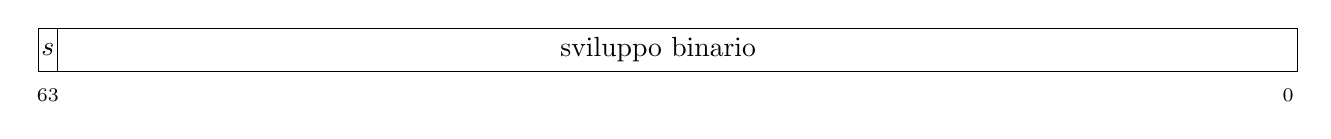
\begin{tikzpicture}[main node/.style={rectangle,draw,inner sep=0.,outer sep=0.}]%
  \pgfmathsetmacro{\xscale}{0.25}
  \pgfmathsetmacro{\yscale}{0.55}
  \draw[draw=black] (0., 0.) rectangle (1. * \xscale, 1. * \yscale);
  \draw[draw=black] (1. * \xscale, 0.) rectangle (64. * \xscale, 1. * \yscale);
  \node at (0.5 * \xscale, 0.5 * \yscale) {$s$};
  \node at (0.5 * \xscale, -0.55 * \yscale) {\scriptsize{$63$}};
  \node at (63.5 * \xscale, -0.55 * \yscale) {\scriptsize{$0$}};
  \node at (31.5 * \xscale, 0.5 * \yscale) {sviluppo binario};
  %\foreach \x in {0,1,...,31}
  %\node[main node] at (\x*\xscale, 0) {0};

  %\foreach \x in {0,1,...,31}
  %\node[main node] at (\x*\xscale, -0.75) {0};
\end{tikzpicture}

  \vspace*{-15pt}
  \caption{Rappresentazione di un numero intero con segno a 64 bit. Il bit
  più significativo è riservato per il segno ($0$ indica un numero
  positivo, $1$ un numero negativo), e gli altri 63 bit contengono lo sviluppo
  binario del valore di partenza.}
  \label{fig:rappresentazione_interi}
\end{figure}

Molti linguaggi di programmazione offrono un controllo granulare sui numeri
interi, fornendo tipi predefiniti a 8, 16, 32 e 64~bit,
nella versione con segno (\foreign{signed}) e senza (\foreign{unsigned}). Ad esempio
un \foreign{unisgned} ad 8~bit può contenere gli interi da $0$ a $255$,
mentre un \foreign{signed} ad 8~bit può contenere gli interi da $-128$ a
$127$. Tutto ciò permette di ottimizzare l'uso della memoria ma, allo stesso
tempo, richiede una qualche attenzione nel far sì che, nel flusso del
programma, una variabile di un determinato tipo non ecceda mai i limiti del
tipo stesso (nel qual caso si hanno problemi di \foreign{overflow} o
\foreign{underflow}). Per completezza, in \python\ la gestione dei tipi interi
è completamente trasparente all'utente ed il linguaggio permette di
rappresentare numeri grandi a piacere allocando automaticamente la quantità
di memoria necessaria---fino all'esaurimento della memoria fisica.


\subsection{Numeri in virgola mobile}

Siamo finalmente arrivati alla parte interessante. Lo standard IEEE 754~\cite{ieee_754},
che è ormai adottato pressoché universalmente, fornisce una prescrizione
per la rappresentazione dei numeri in virgola mobile in logica binaria, e
due specifiche di formato: a 32~bit (in precisione singola) e 64~bit (in
precisione doppia), come mostrato in figura~\ref{fig:rappresentazione_float}.
Più precisamente, ogni volta che scriviamo un numero in virgola mobile, dobbiamo
pensare che, all'interno del calcolatore, esso è rappresentato come
\begin{align}\label{eq:ieee_754}
  x = (-1)^s \times m \times 2^{e - b} \quad \text{dove} \quad 1 \leq m < 2,
\end{align}
in cui, spostandosi da sinistra a destra nella rappresentazione---ovverosia dal
bit più significativo a quello meno significativo:
\begin{itemize}
  \item $s$ rappresenta il \emph{segno} del numero, e corrisponde al bit
    più significativo ($0$ se il numero è positivo, $1$ se è negativo);
  \item $e$ è l'esponente, che ha a disposizione 8~bit in precisione singola
    e 11~bit in precisione doppia; $b$, che prende il nome di \foreign{bias},
    è una costante additiva (positiva) che permette di rappresentare numeri
    $< 1$ senza bisogno di aggiungere un segno all'esponente, e vale $127$ in
    precisione singola e $1023$ in precisione doppia;
  \item $m$ prende il nome di \emph{mantissa} e rappresenta (utilizzando 23~bit in
    precisione singola e 52~bit in precisione doppia) la sequenza di cifre dopo
    la virgola, \emph{assumendo che la parte intera sia $1$} (cioè la mantissa
    è convenzionalmente compresa tra $1$ e $2$ ed il bit più significativo,
    che è garantito essere $1$, può essere omesso).
\end{itemize}

\begin{figure}[!htbp]
  \center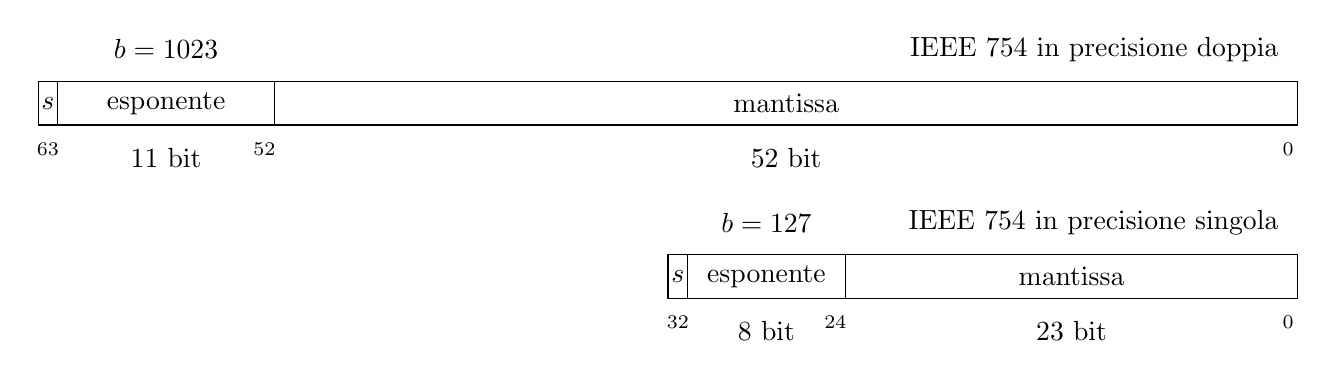
\begin{tikzpicture}[main node/.style={rectangle,draw, inner sep=0.,outer sep=0.}]%
  \pgfmathsetmacro{\xscale}{0.25}
  \pgfmathsetmacro{\yscale}{0.55}
  \draw[draw=black] (0., 0.) rectangle (1. * \xscale, 1. * \yscale);
  \draw[draw=black] (1. * \xscale, 0.) rectangle (12. * \xscale, 1. * \yscale);
  \draw[draw=black] (12. * \xscale, 0.) rectangle (64. * \xscale, 1. * \yscale);
  \node at (0.5 * \xscale, 0.5 * \yscale) {$s$};
  \node at (0.5 * \xscale, -0.55 * \yscale) {\scriptsize{$63$}};
  \node at (11.5 * \xscale, -0.55 * \yscale) {\scriptsize{$52$}};
  \node at (63.5 * \xscale, -0.55 * \yscale) {\scriptsize{$0$}};
  \node at (6.5 * \xscale, 0.5 * \yscale) {esponente};
  \node at (38. * \xscale, 0.5 * \yscale) {mantissa};
  \node[anchor=east] at (63.5 * \xscale, 1.75 * \yscale) {IEEE 754 in precisione doppia};
  \node at (6.5 * \xscale, 1.75 * \yscale) {$b=1023$};
  \node at (6.5 * \xscale, -0.75 * \yscale) {$11$~bit};
  \node at (38. * \xscale, -0.75 * \yscale) {$52$~bit};

  \draw[draw=black] (32. * \xscale, -4. * \yscale) rectangle (33. * \xscale, -3. * \yscale);
  \draw[draw=black] (33. * \xscale, -4. * \yscale) rectangle (41. * \xscale, -3. * \yscale);
  \draw[draw=black] (41. * \xscale, -4. * \yscale) rectangle (64. * \xscale, -3. * \yscale);
  \node at (32.5 * \xscale, -3.5 * \yscale) {$s$};
  \node at (32.5 * \xscale, -4.55 * \yscale) {\scriptsize{$32$}};
  \node at (40.5 * \xscale, -4.55 * \yscale) {\scriptsize{$24$}};
  \node at (63.5 * \xscale, -4.55 * \yscale) {\scriptsize{$0$}};
  \node at (37.0 * \xscale, -3.5 * \yscale) {esponente};
  \node at (52.5 * \xscale, -3.5 * \yscale) {mantissa};
  \node[anchor=east] at (63.5 * \xscale, -2.25 * \yscale) {IEEE 754 in precisione singola};
  \node at (37.0 * \xscale, -2.25 * \yscale) {$b=127$};
  \node at (37. * \xscale, -4.75 * \yscale) {$8$~bit};
  \node at (52.5 * \xscale, -4.75 * \yscale) {$23$~bit};

\end{tikzpicture}

  \vspace*{-10pt}
  \caption{\foreign{Layout} dei due formati per la rappresentazione binaria dei
  numeri in virgola mobile definiti dallo standard IEEE~754: in precisione
  doppia (11~bit per l'esponente e 53 per la mantissa) ed in precisione singola
  (8~bit per l'esponente e 23 per la mantissa). Il \foreign{bias} per l'esponente
  è $1023$ nel primo caso e $127$ nel secondo.}
  \label{fig:rappresentazione_float}
\end{figure}


Cominciamo allora da un numero semplice (i.e., con uno sviluppo binario finito,
come quello che abbiamo considerato all'inizio di questa sezione):
\begin{align*}
  x = 2.25 = 0b10.01 = \frac{9}{4} = 1.125 \times 2.
\end{align*}
I passaggi sono tutti rilevanti (e.g., $\nicefrac{9}{4}$ costituisce la
rappresentazione di $x$ come il rapporto tra i due interi più piccoli possibile,
come potete verificare direttamente utilizzando \pyfunc{as_integer_ratio} in \python)
ma l'ultimo è quello più importante, perché rappresenta $x$ esattamente
nella forma~\eqref{eq:ieee_754}, ovverosia come il prodotto di una mantissa
$1 \leq m < 2$ per una potenza di $2$.
Nel formato in doppia precisione avremo dunque
\begin{align*}
  s & = 0\\
  e & - b = 1 \implies e = 1024 =  0b10000000000\\
  m & = 1.125 = 0b(1).0010000000000000000000000000000000000000000000000000
\end{align*}
(notate che abbiamo indicato tutti gli 11~bit per l'esponente ed i 52~per la
mantissa, con il bit più significativo di normalizzazione tra parentesi) e,
in definitiva
\begin{align*}
  x \rightarrow 0b0\overbrace{0010000000}^{e-b}
  \overbrace{0010000000000000000000000000000000000000000000000000}^{m~\text{(bit più significativo omesso)}}
  = 0x4002000000000000 .
\end{align*}
Wow! Abbiamo scritto il nostro primo numero in virgola mobile nella forma in
cui lo troveremmo nel disco rigido del nostro calcolatore! Adesso possiamo
chiudere il cerchio e provare a fare la stessa cosa con il famigerato
\begin{align*}
  x = 0.1 = 0.1 \times 16 \times 2^{-4} = 1.6 \times 2^{-4}.
\end{align*}
Procedendo esattamente come prima si ha
\begin{align*}
  s & = 0 \\
  e & - b = - 4 \implies e = 1019 = 0b01111111011\\
  m & = 1.6 \approx 0b(1).1001100110011001100110011001100110011001100110011010
\end{align*}
(notate che questa volta la mantissa non può rappresentare esattamente il numero di
partenza con un numero finito di bit) e dunque
\begin{align*}
  x \rightarrow 0b0\overbrace{01111111011}^{e-b}
  \overbrace{1001100110011001100110011001100110011001100110011010}^{m~\text{(bit più significativo omesso)}}
  = 0x3FB999999999999A.
\end{align*}
La cosa interessante, a questo punto, è che se moltiplichiamo la mantissa per
$2^{52}$ (il che equivale a considerare la mantissa stessa, incluso il bit più
significativo \emph{nascosto}, come un numero intero espresso in base $2$), si ha
\begin{align*}
  x = \frac{m \times 2^{52}}{2^{52 - (e  - b)}} =
  \frac{7205759403792794}{2^{56}} = \frac{3602879701896397}{2^{55}}
\end{align*}
(l'ultimo passaggio è possibile grazie al fatto che il numeratore è divisibile
per $2$, in quanto la cifra meno significativa del suo sviluppo binario è zero).
Ricorda qualcosa? Il frammento~\ref{snip:integer_ratio}?


\section{Buone e cattive proprietà dell'aritmetica in virgola mobile}

Adesso che abbiamo gli strumenti di base per una discussione più informata sulle
proprietà dell'aritmetica in virgola mobile su un calcolatore digitale,
facciamo un passo indietro e riesaminiamo criticamente alcune delle cose che
abbiamo detto all'inizio di questa sezione.

Il modello di rappresentazione dei numeri codificato nello standard IEEE~754
ha una serie di buone proprietà che lo rendono estremamente versatile e
riducono, per quanto possibile, il potenziale impatto della precisione finita
sui risultati finali: permette di rappresentare numeri su un intervallo dinamico
di molti ordini di grandezza e fornisce la stessa accuratezza \emph{relativa}
su tutto l'intervallo. In particolare: il massimo numero rappresentabile è dettato
da numero di bit $n_e$ dell'esponente
\begin{align*}
  x_\text{max} \approx 2^{2^{n_e - 1}} =
  \begin{cases}
    2^{128} \approx 10^{38} \quad & \text{in precisione singola}\\
    2^{1024} \approx 10^{308} \quad & \text{in precisione doppia}.
  \end{cases}
\end{align*}
Se si considera che il numero stimato di protoni nell'universo è dell'ordine di
$10^{80}$ e la lunghezza di Planck è $1.6 \times 10^{-35}$~m, capiamo
immediatamente che non c'è di che preoccuparsi.

Di converso, la \emph{precisione} è dettata dal numero $n_m$ di bit a disposizione
per la mantissa, e si può esprimere in termini di cifre decimali equivalenti
come
\begin{align*}
  \frac{x}{\varepsilon_x} \approx \log_{10} \left( 2^{n_s + 1}\right) =
  \begin{cases}
    7 \quad & \text{in precisione singola}\\
    16 \quad & \text{in precisione doppia}.
  \end{cases}
\end{align*}
Anche qui, almeno apparentemente, non abbiamo niente da temere---il momento magnetico
dell'elettrone è misurato in circa una parte su $10^{12}$, e questo
rappresenta più o meno lo stato dell'arte.

\snip{floating_point2}{%
Semplice illustrazione di come la proprietà commutativa dell'addizione non
valga quando applicata all'aritmetica in virgola mobile su un calcolatore
digitale.}

Eppure non possiamo chiudere gli occhi e riposare tranquilli, perché l'aritmetica in
virgola mobile è prodiga di sorprese, come mostrato nel frammento di
codice~\ref{snip:floating_point2}. La referenza~\cite{bush_floating_point}
contiene una discussione più approfondita della questione ed una serie di consigli
pratici per evitare i problemi più comuni (e.g., sottrazione di numeri molto grandi
vicini tra loro, operazioni con numeri che differiscono di molti ordini di grandezza,
confronto tra numeri in virgola mobile nel controllo del flusso logico del programma),
ma adesso è veramente giunto il momento di chiudere.
